\subsubsection{13.02.15 (Соревнования)}
\begin{center}
	3-ий день соревнований "Робофест-7 в Москве"
\end{center}
Сегодня проходили финальные матчи.\newline

Утром, до объявления результатов квалификационных матчей, мы еще раз поговорили со всеми участниками соревнований и рассказали им о преимуществах, которые они получат, выбрав к себе в альянс именно нашу команду. Таким образом мы постарались увеличить свои шансы быть выбранными в альянс в том случае, если мы не попадем в топ-4 лучших команд и не сможем выбирать союзников по альянсу сами.\newline

Когда объявили результаты квалификационных матчей, оказалось, что наша команда была на 4 месте в рейтинге. Мы получили возможность выбирать себе союзников в альянс. Поскольку это крупные соревнования, в альянсы набиралось по 3 команды (на всех предыдущих соревнованиях, на которых мы были, альянсы состояли из 2 команд). Мы отказались от предложения вступить в альянс с командой FTC-5, занявшей 3 место в рейтинге, и выбрали команды FTC-22 (с которой мы сыграли очень результативный матч во время квалификационных заездов) и FTC-10 (которая могла в одиночку наполнить корзину 90 см за матч).\newline

В полуфинале мы выиграли обе игры, первую в паре с командой FTC-22, а вторую - в паре с FTC-10.\newline

В финале мы играли против альянса, одна из команд которого имела автономную программу, в ходе которой он передвигал наши подвижные корзины и делал невозможным взаимодействие с ними. Поэтому во второй игре, когда со стороны альянса-противника выступал описанный робот, мы решили не участвовать в игре лично, так как наш автоном в данном случае бессилен, а поставить на игру команды 22 и 10. Рассчет оказался верным, команда 22 в автономном периоде смогла сбить палку-упор и получить 30 очков, в то время как противник не получил ничего за автономный период. Вторая игра закончилась нашей победой. Первую же игру мы выиграли в паре с 10-ой командой.\newline

Таким образом, наш альянс стал победителем фестиваля в категории FIRST FTC.\newline

Внесенные доработки:
\begin{enumerate}
	\item Для того, чтобы движение нашего робота в автономном периоде не помешало нашему союзнику по альянсу, команде FTC-10 (они съезжали с пандуса и закидывали два автономных мяча в корзину 60 см), мы изменили траекторию движения к зоне парковки.
	\begin{figure}[H]
		\begin{minipage}[h]{0.2\linewidth}
			\center  
		\end{minipage}
		\begin{minipage}[h]{0.6\linewidth}
			\center{\includegraphics[scale=0.4]{days/13.02.15/images/01}}
			\caption{}
		\end{minipage}
	\end{figure}
	
\end{enumerate}

Результаты соревнований:
\begin{enumerate}
	\item По результатам квалификационных матчей мы заняли в рейтинге 4-е место.
	
	\item Наш альянс одержал победы в полуфинале и финале.
	
	\item Наша команда заняла первое место в общекомандном зачете.
	
	\item В номинации "Защита инженерной книги" призовых мест мы не заняли.
	
	\item В других номинациях мы также не заняли призовых мест.
\end{enumerate}

Подведение итогов:
\begin{enumerate}
	\item Успешность выступления на соревнованиях:
	\begin{enumerate}
		\item Мы заняли первое место в общекомандном зачете и получили право представлять Россию на международных соревнованиях FIRST FTC, которые будут проводиться в апреле в Сент-Луисе, США.
		
		\item Из 7 игр, которые мы сыграли (4 в квалификации и 3 в финале), мы одержали победу в 6.
		
		\item Благодаря тренировкам на этих соревнованиях наши операторы успешно управляли роботом, работали слаженно и грамотно координировали свои действия как друг с другом, так и с операторами союзных команд.
		
		\item Механическая составляющая робота работала стабильно и не ломалась на протяжении всех матчей (в отличие от предыдущих соревнований).
		
		\item Программа автономного периода работала стабильно, но давала в среднем только половину изначально запланированных очков.
		
		\item Программа управляемого периода сбоев не давала.
		
	\end{enumerate}
	
	\item Наши ошибки и недостатки конструкции:
	\begin{enumerate}
		\item Несмотря на то, что ранее мы реализовали промежуточное положение ковша, застревание мячей по-прежнему оставалось серьезной проблемой, из-за которой мы теряли много времени на закидывание мячей в корзину.
		
		\item Из-за того, что пандус для мячей является частью ковша, когда ковш поднимается, мы не можем ехать вперед к новой куче больших мячей, потому что в этом случае маленькие мячи будут закатываться под робота. Если мы сделаем пандус отдельным от ковша стационарным элементом, то эта проблема будет решена.
		
	\end{enumerate}
	
	\item Полезные технические решения, которые мы почерпнули у других команд:
	\begin{enumerate}
		\item Робот одной из команд на соревнованиях имел приспособление, при помощи которого он мог поднимать подвижную корзину над полем. Это позволяло ему получить 30 очков за отрыв корзины от земли в финале не завозя ее на пандус.
		\begin{figure}[H]
			\begin{minipage}[h]{0.2\linewidth}
				\center  
			\end{minipage}
			\begin{minipage}[h]{0.6\linewidth}
				\center{\includegraphics[scale=0.25]{days/13.02.15/images/02}}
				\caption{Захват для корзин}
			\end{minipage}
		\end{figure}
		
		\item Робот команды из Румынии имел ходовую, состоящую из 6 обычных колес, способных поворачиваться вокруг вертикальной оси, что давало ему возможность двигаться боком и по диагонали, но при этом избежать проблем, свойственных роботам на омни-колесах - проскальзывания и неточности движения по энкодерам в автономном периоде а также проблем с заездом на пандус.
		\begin{figure}[H]
			\begin{minipage}[h]{0.2\linewidth}
				\center  
			\end{minipage}
			\begin{minipage}[h]{0.6\linewidth}
				\center{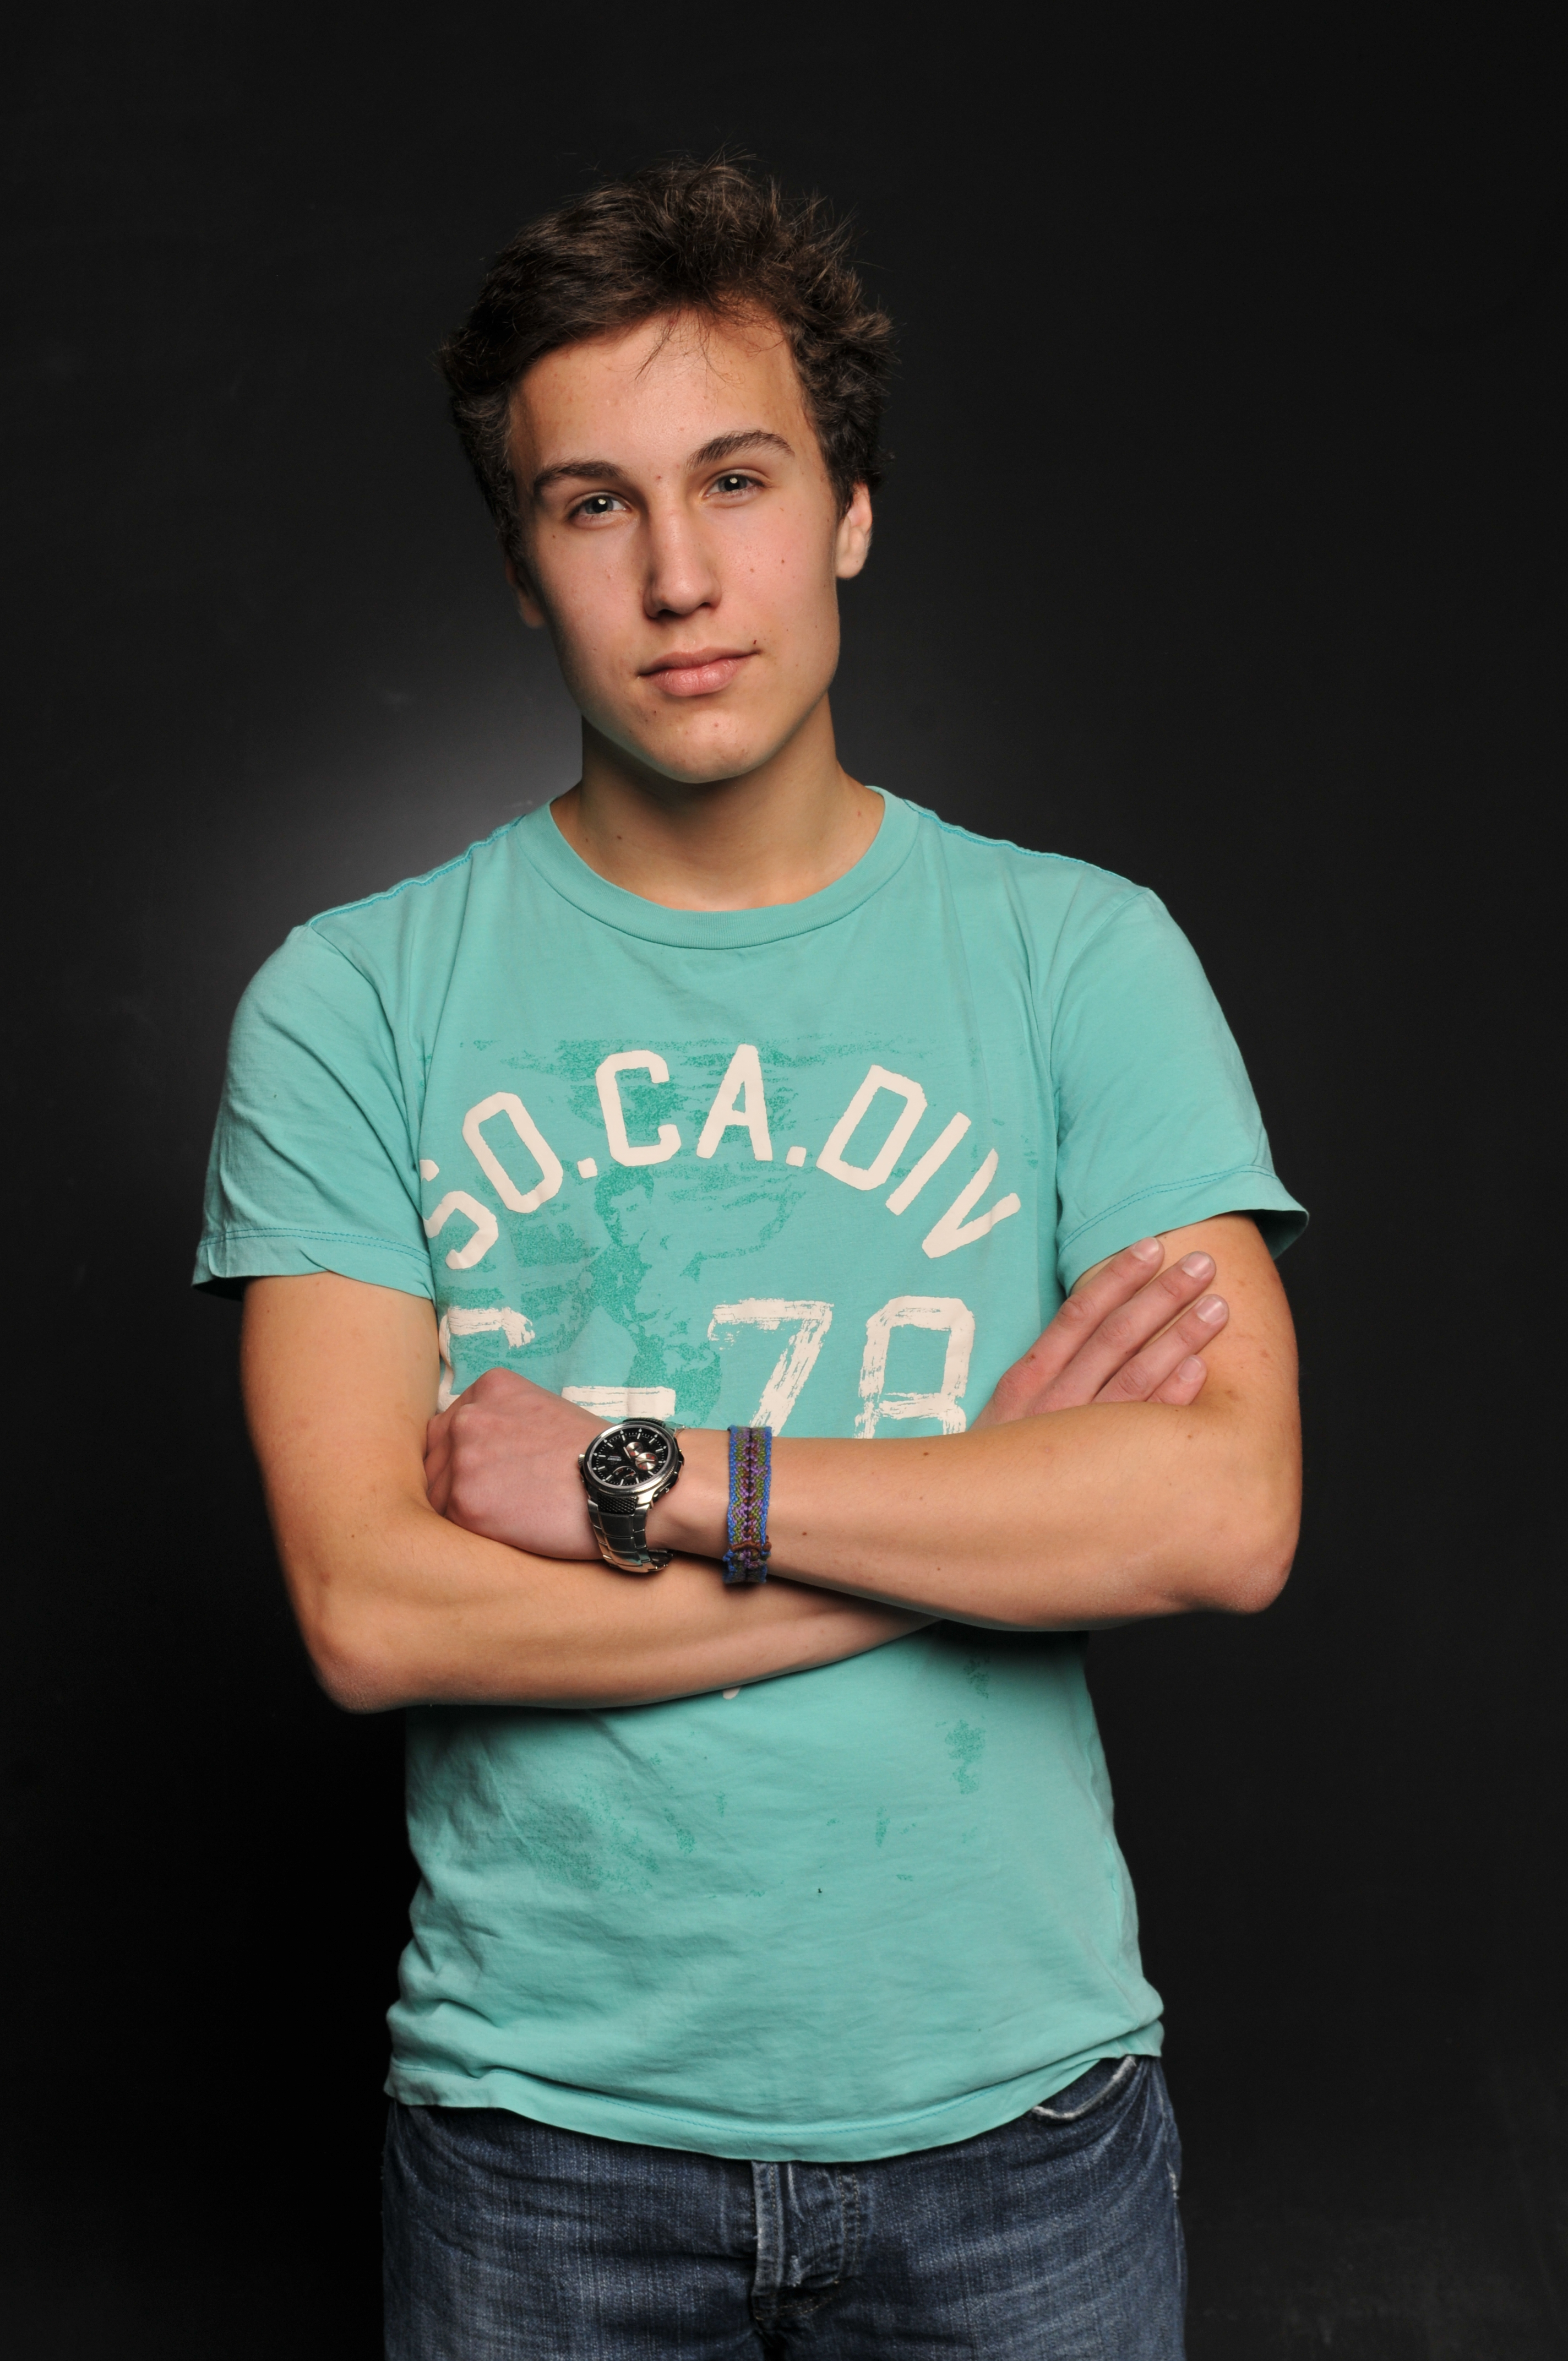
\includegraphics[scale=0.2]{days/13.02.15/images/03}}
				\caption{Робот румынской команды (устройство ходовой не показано)}
			\end{minipage}
		\end{figure}
		
		\item Один из роботов имел специальные клешнеобразные захваты, с помощью которых он сгребал мячи в кучу и подгонял их к главному захвату, закидывающему мячи в ковш. Эта конструкция была особенно эффективна в том случае, когда мячи располагались у бортика и основной захват мог с трудом до них достать.
		\begin{figure}[H]
			\begin{minipage}[h]{0.47\linewidth}
				\center{\includegraphics[scale=0.2]{days/13.02.15/images/04}}
			\end{minipage}
			\hfill
			\begin{minipage}[h]{0.47\linewidth}
				\center{\includegraphics[scale=0.21]{days/13.02.15/images/05}}
			\end{minipage}
			\caption{Клешнеобразные захваты}
		\end{figure}
		
	\end{enumerate}
	
	\item Задачи для последующих собраний:
	\begin{enumerate}
		\item Реализовать механизм, позволяющий поднимать подвижную корзину над землей.
		
		\item Реализовать программу автономного периода, с ориентацией по ИК-датчику, так как помешать работе такого автонома противник не сможет.
		
		\item Реализовать ориентацию робота на поле по компасу, так как он точнее, чем энкодеры при поворотах.
		
		\item Создать клешнеобразный захват для мячей, помогающий основному захвату собирать мячи.
		
		\item Сделать 3D модель робота в Creo как можно более точной и детальной.
		
		\item Реализовать механизм, препятствующий застреванию больших мячей в ковше.
			
		\item Сделать пандус для закидывания мячей в ковш стационарным.
		
		\item Увеличить мощность механизма опрокидывания ковша таким образом, чтобы он мог опрокидывать ковш с 5 мячами одновременно.
		
	\end{enumerate}
	
	\item Поскольку следующие наши соревнования пройдут в Сент-Луисе, вся последующая документация будет вестись исключительно на английском языке.
	
\end{enumerate}
\fillpage